\documentclass{article}
\usepackage[utf8]{inputenc}
\usepackage{graphicx} % Per le immagini
\usepackage{caption} % Per didascalie personalizzate
\usepackage{subcaption} % Per sottofigure
\usepackage{float}

\title{Relazione del Progetto di Programmazione Web e Mobile}
\author{Francesco Franguelli Emanuele}

\begin{document}

\maketitle

\section*{Introduzione}
Il progetto "Album delle Figurine di Harry Potter (AFHP)" è un'applicazione web per la gestione di un album elettronico di figurine di super eroi. Il progetto prevede la gestione del profilo utente, l'acquisto (simulato) di crediti e pacchetti di figurine, e la gestione dello scambio di figurine tra giocatori.

\section{Configurazione e avvio dell'applicazione}
    Per eseguire l'app bisogna seguire i seguenti passagggi:
    \begin{itemize}
        \item scaricare il codice sorgente
        \item aver installato node js e npm
        \item installare le dipendenze con il comando 'npm install'
        \item configurare correttamente il file .env (il file .env è gia presente nel codice sorgente ed è gia impostato, ma se da problemi occorre riconfiguralo addeguatamente)
        \item avviare il progetto con il comando 'npm run start'
        \item a questo punto si può accedere al sito web al link "https://127.0.0.1:3000" (attenzione questo è il link di default se è stato modificato il file .env il link potrebbe differire)
        \item una volta effettuato l'accesso il browser potrebbe segnalare il sito come non sicuro in quanto i certificati per l'https sono stati autofirmati, bastera chiudere il pop up e si potra accedere al sito, in alternativa si possono cambiare i certificati con dei certificati validi.
    \end{itemize}

\section{Struttura}
    Il progetto è suddiviso in 3 cartelle principali:
    \begin{itemize}
        \item \textbf{FrontEnd}: questa cartella contiene tutto il codice del sito web che viene eseguito lato client. Al suo interno troviamo 3 cartelle: \texttt{html}, \texttt{css}, \texttt{javascript}, che contengono i vari file del sito web.
        \item \textbf{BackEnd}: in questa cartella è presente tutto il codice del backend, ovvero le API. Al suo interno troviamo il file \texttt{routes.js}, in cui sono scritti i vari endpoint delle API, ciascuno associato al controller, cioè la funzione che gestisce la richiesta. La cartella \texttt{middleware} contiene il file \texttt{auth.js}. I middleware sono funzioni che gestiscono alcune richieste, ma non forniscono la risposta. Piuttosto, effettuano una prima parte di elaborazione. In questo caso, \texttt{auth.js} si occupa di verificare se la richiesta proviene da un utente autenticato e, successivamente, passa la richiesta al controller di competenza. Infine, c'è la cartella \texttt{controllers}, che contiene i file dei vari controller, suddivisi in \texttt{user} (controller che gestiscono le operazioni sugli utenti), \texttt{trade} (controller che gestiscono le operazioni di scambio) e \texttt{marvel} (controller che utilizzano le API esterne di Marvel).
        \item \textbf{Database}: questa cartella contiene il file \texttt{database.js}, che si occupa della connessione al database, e la cartella \texttt{schemas}, che contiene gli schemi del progetto.
    \end{itemize}
    
    Oltre a queste 3 cartelle, ci sono altri file e cartelle importanti:
    \begin{itemize}
        \item Il file \texttt{server.js}, che viene eseguito all'avvio del progetto e si occupa di connettersi al database e successivamente di avviare il server.
        \item La cartella \texttt{docs}, che contiene la documentazione del progetto.
        \item La cartella \texttt{certificate}, che contiene i certificati.
        \item Altri file, come la cartella \texttt{node\_modules}, che contiene le dipendenze del progetto, e file di configurazione come \texttt{.gitignore}.
    \end{itemize}


\section{Progettazione}
Il progetto è stato sviluppato come un server HTTPS che ospita un sito web dedicato alle figurine, con le relative API disponibili alla root \texttt{/api/...}. La connessione al database avviene prima dell'avvio del server. Il database scelto è MongoDB, un database NoSQL, e la sua gestione avviene nel cloud tramite MongoDB Atlas.

Per ottenere informazioni sulle figurine, sono utilizzate le API pubbliche. L'autenticazione degli utenti avviene tramite cookie, che vengono inviati con le richieste quando necessario. In particolare, viene utilizzato un token JWT (JSON Web Token) per gestire l'autenticazione degli utenti.

    
\section*{Implementazione}

    \subsection*{Sito Web}
    La parte relativa al sito web è stata sviluppata utilizzando il framework \textit{Bootstrap}, che fornisce una griglia flessibile e componenti predefiniti per la creazione di interfacce utente reattive. Questo framework consente di adattare automaticamente l'interfaccia a diverse risoluzioni e dispositivi, garantendo un'esperienza utente ottimale su desktop, tablet e dispositivi mobili. 
    
    La struttura del sito è stata progettata per essere semplice, chiara e intuitiva, con una navigazione fluida e facilmente accessibile. Per la visualizzazione delle figurine e delle informazioni correlate, sono stati utilizzati vari componenti di Bootstrap, come modali, pulsanti e tabelle, che semplificano l'interazione con il contenuto.
    
    Il sito è ospitato su un server principale che utilizza Express per gestire le richieste HTTP e servire i contenuti dinamici, consentendo un'interazione rapida ed efficiente con l'utente.
    
    \subsection*{Interazione con le API}
    Il sito web interagisce con il backend tramite API RESTful, che permettono di recuperare i dati relativi alle figurine e di gestire le operazioni di autenticazione. Le API sono state sviluppate utilizzando Express e il modulo \textit{swagger-ui-express}, che consente di visualizzare facilmente la documentazione delle API in modo chiaro e intuitivo per gli sviluppatori.
    
    Il backend accede al database tramite \textit{Mongoose}, una libreria che facilita l'interazione con MongoDB utilizzando schemi e modelli. Questo approccio semplifica lo sviluppo e consente una gestione più organizzata e strutturata dei dati, garantendo al contempo un'integrazione fluida tra il database e le API.
    
    \subsection*{Autenticazione e Sicurezza}
    L'autenticazione degli utenti è gestita tramite token JWT (JSON Web Token), che vengono inviati con ogni richiesta al backend per garantire l'accesso alle risorse protette. I cookie contenenti i token JWT vengono generati dal backend e utilizzati per validare l'identità dell'utente in modo sicuro, mantenendo la sessione attiva durante la navigazione.
    
    Per proteggere il sito web da vulnerabilità comuni, come Cross-Site Scripting (XSS) e Cross-Site Request Forgery (CSRF), sono state adottate le necessarie misure di sicurezza. Tra queste, la gestione sicura dei cookie e l'uso di HTTPS per crittografare le comunicazioni tra client e server, garantendo così la protezione dei dati sensibili e la privacy degli utenti.
    
\section{Funzionalità Implementate (tra quelle a scelta)}
    Ho deciso di implementare le seguenti funzionalità:
    
    \begin{itemize}
        \item \textbf{Estensione del baratto}: è stata introdotta la possibilità di effettuare scambi più complessi, come ad esempio scambiare due figurine per una, ampliando così le opzioni di scambio disponibili.
        \item \textbf{Vendita di figurine}: gli utenti possono ora vendere le figurine in loro possesso in cambio di crediti, che possono essere utilizzati per acquisire altre figurine o per altre funzionalità del sistema.
        \item \textbf{Controlli di integrità}: sono stati implementati dei controlli per evitare che gli utenti ricevano figurine già in loro possesso o propongano scambi che includano due o più figurine uguali, garantendo così una gestione più equa e logica degli scambi.
    \end{itemize}

\section*{Test e Validazione}
    Di seguito alcuni screenshot del sito web in esecuzione. Le immagini mostrano le varie schermate dell'applicazione, inclusa la home page, la pagina di login, la registrazione, la visualizzazione dei crediti, l'acquisto di pacchetti di figurine, la visualizzazione dell'album e la gestione degli scambi.
    \begin{figure}[H]
        \centering
        \begin{minipage}{0.3\linewidth}
            \centering
            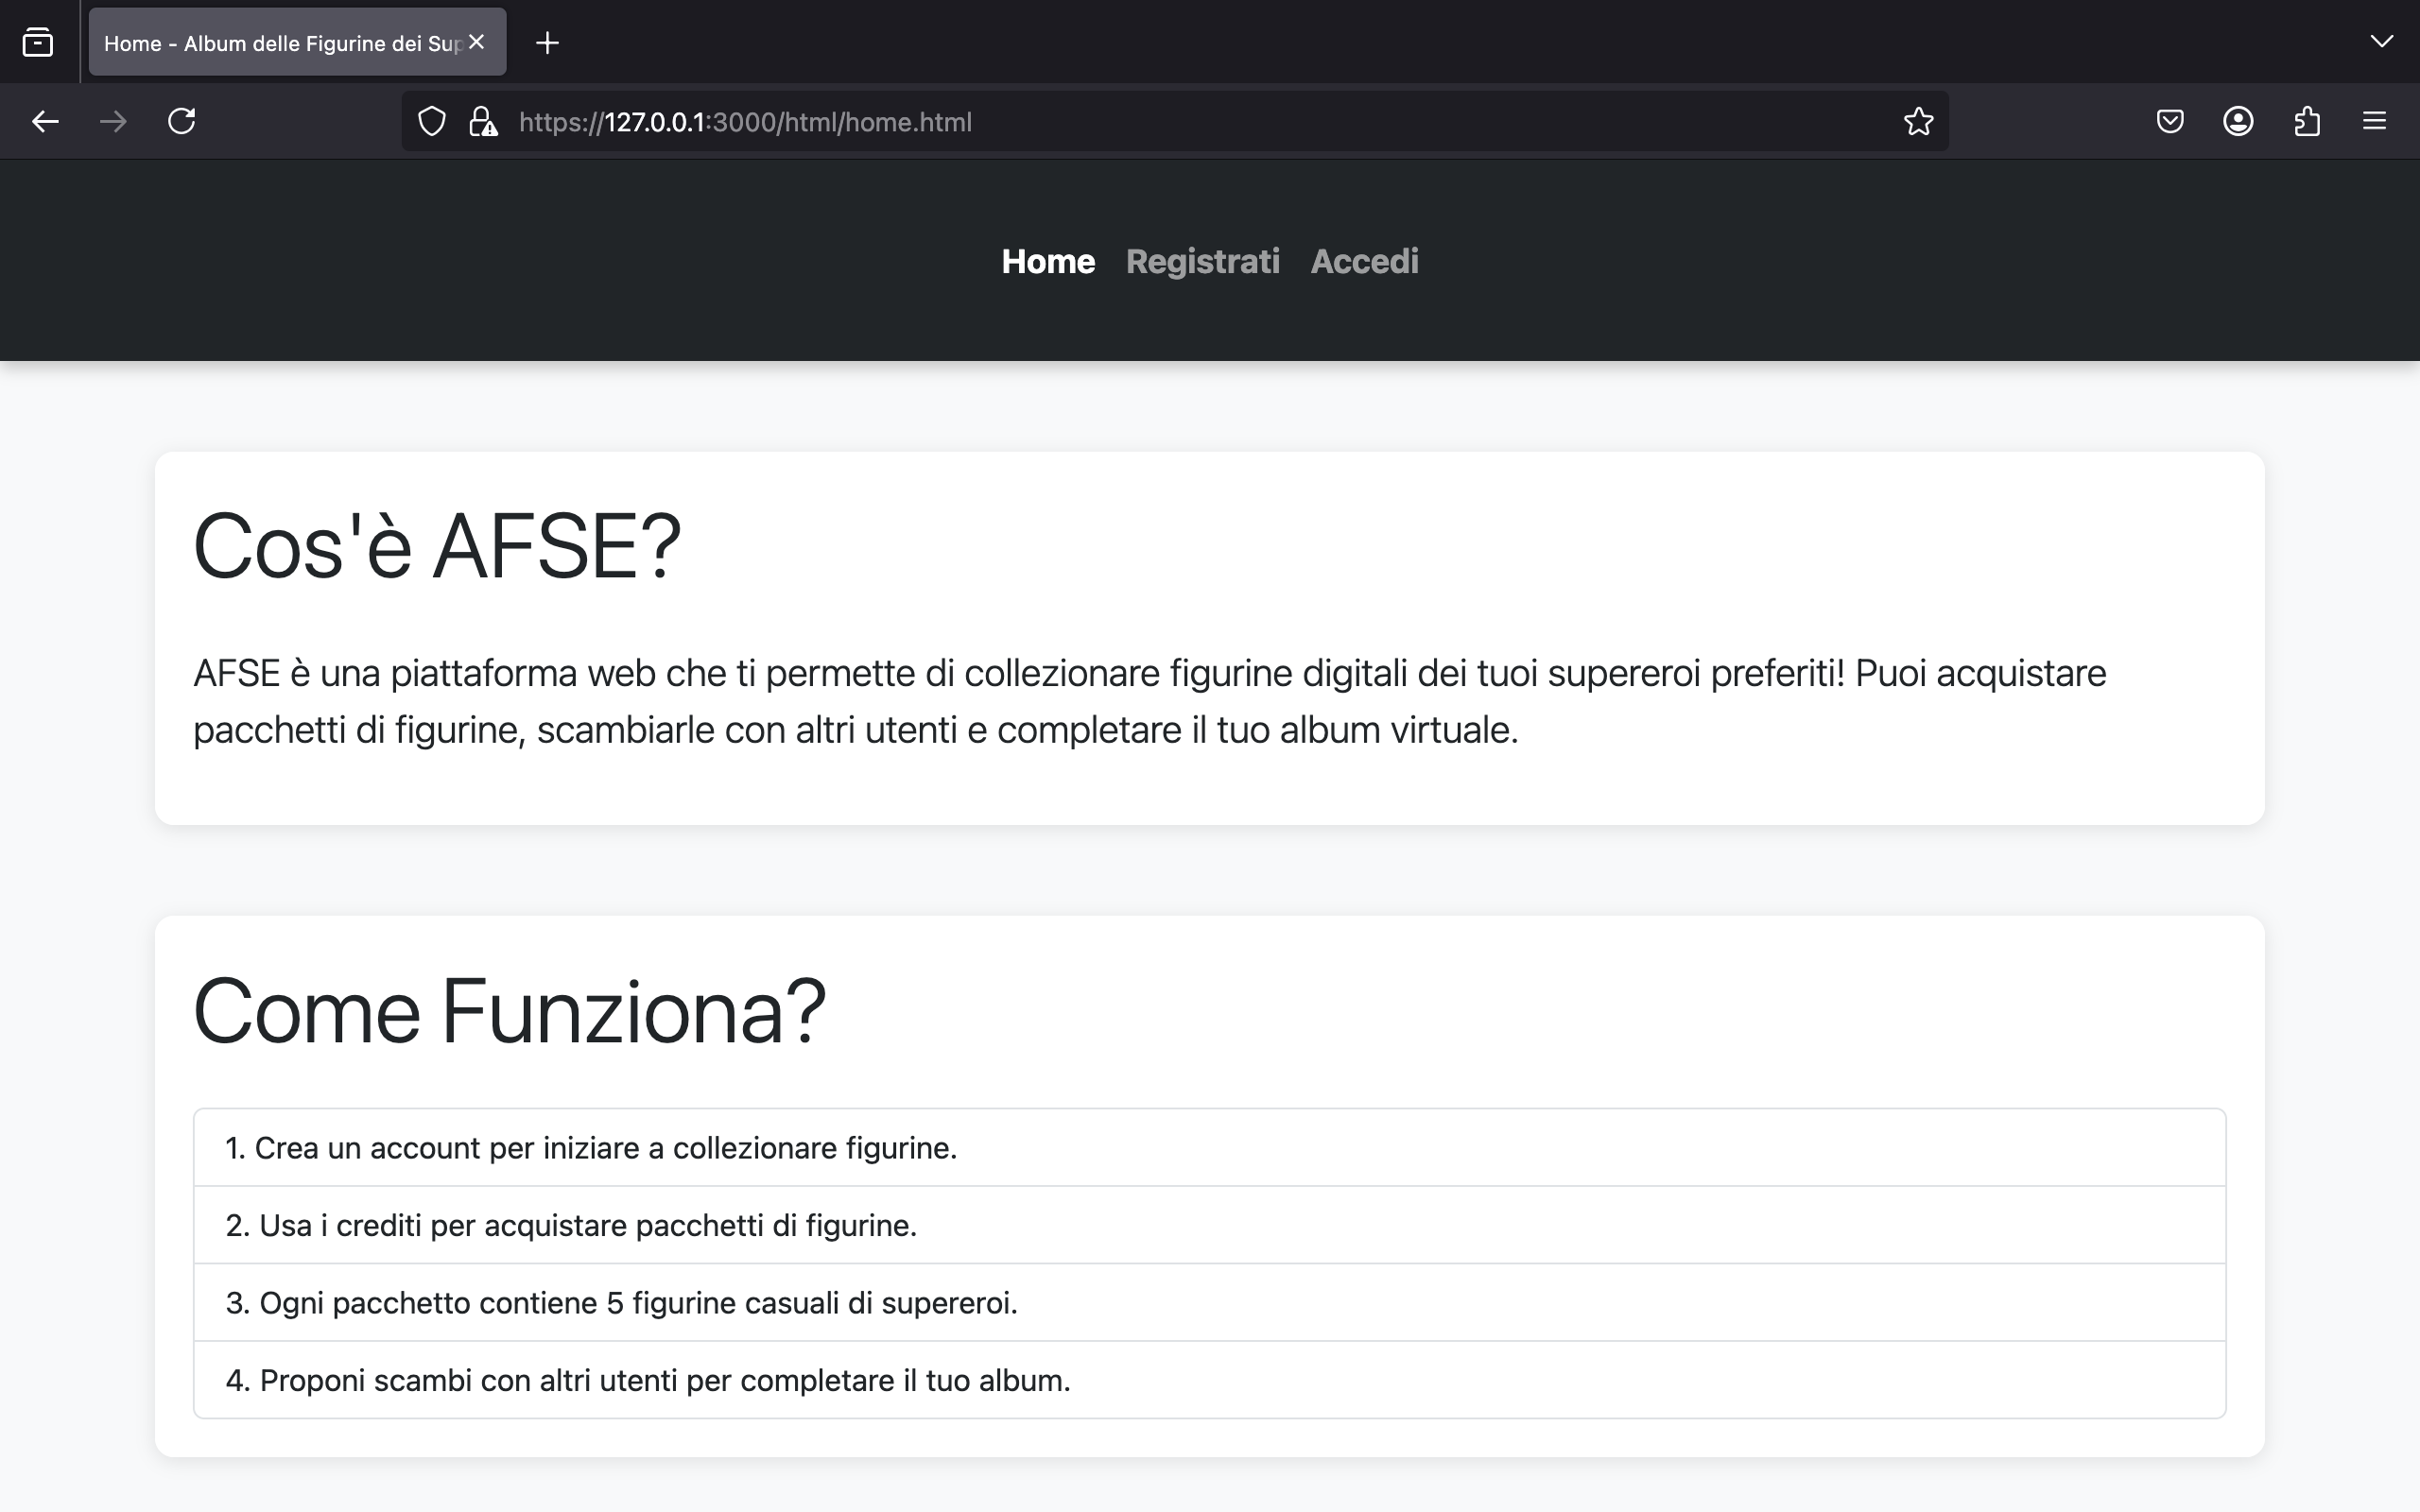
\includegraphics[width=\linewidth]{./content/home.png}
        \end{minipage}
        \hfill
        \begin{minipage}{0.3\linewidth}
            \centering
            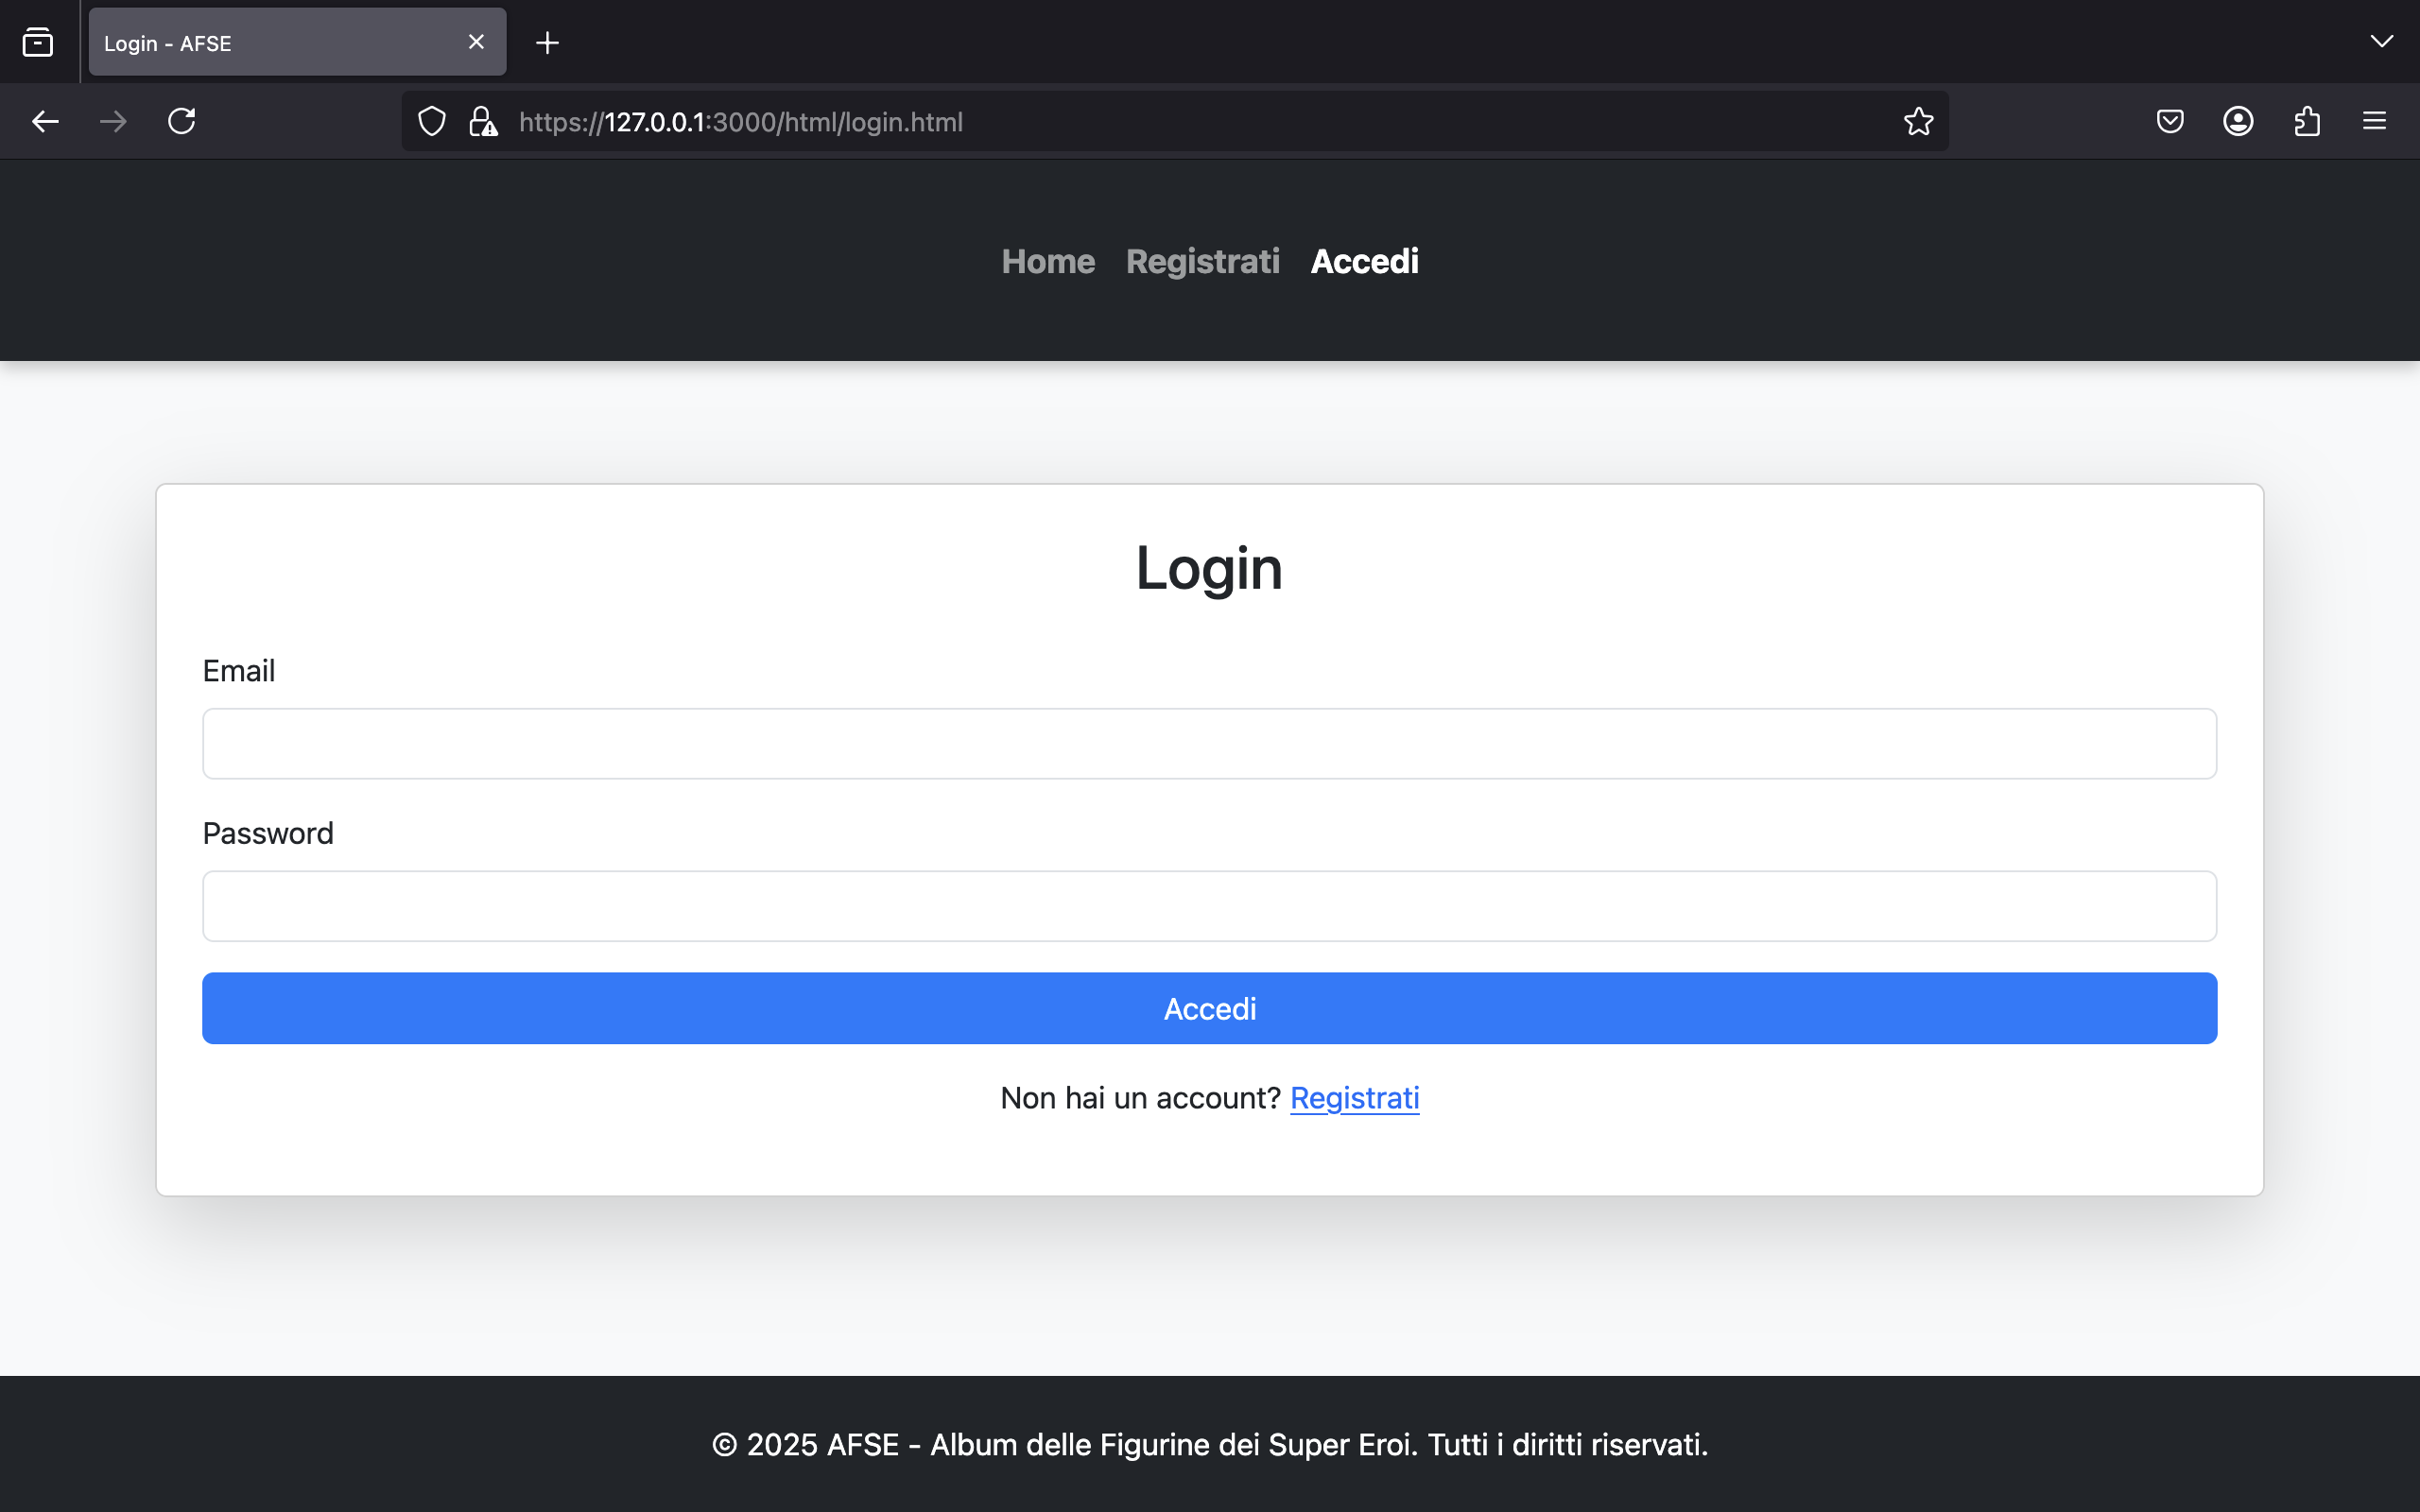
\includegraphics[width=\linewidth]{./content/login.png}
        \end{minipage}
        \hfill
        \begin{minipage}{0.3\linewidth}
            \centering
            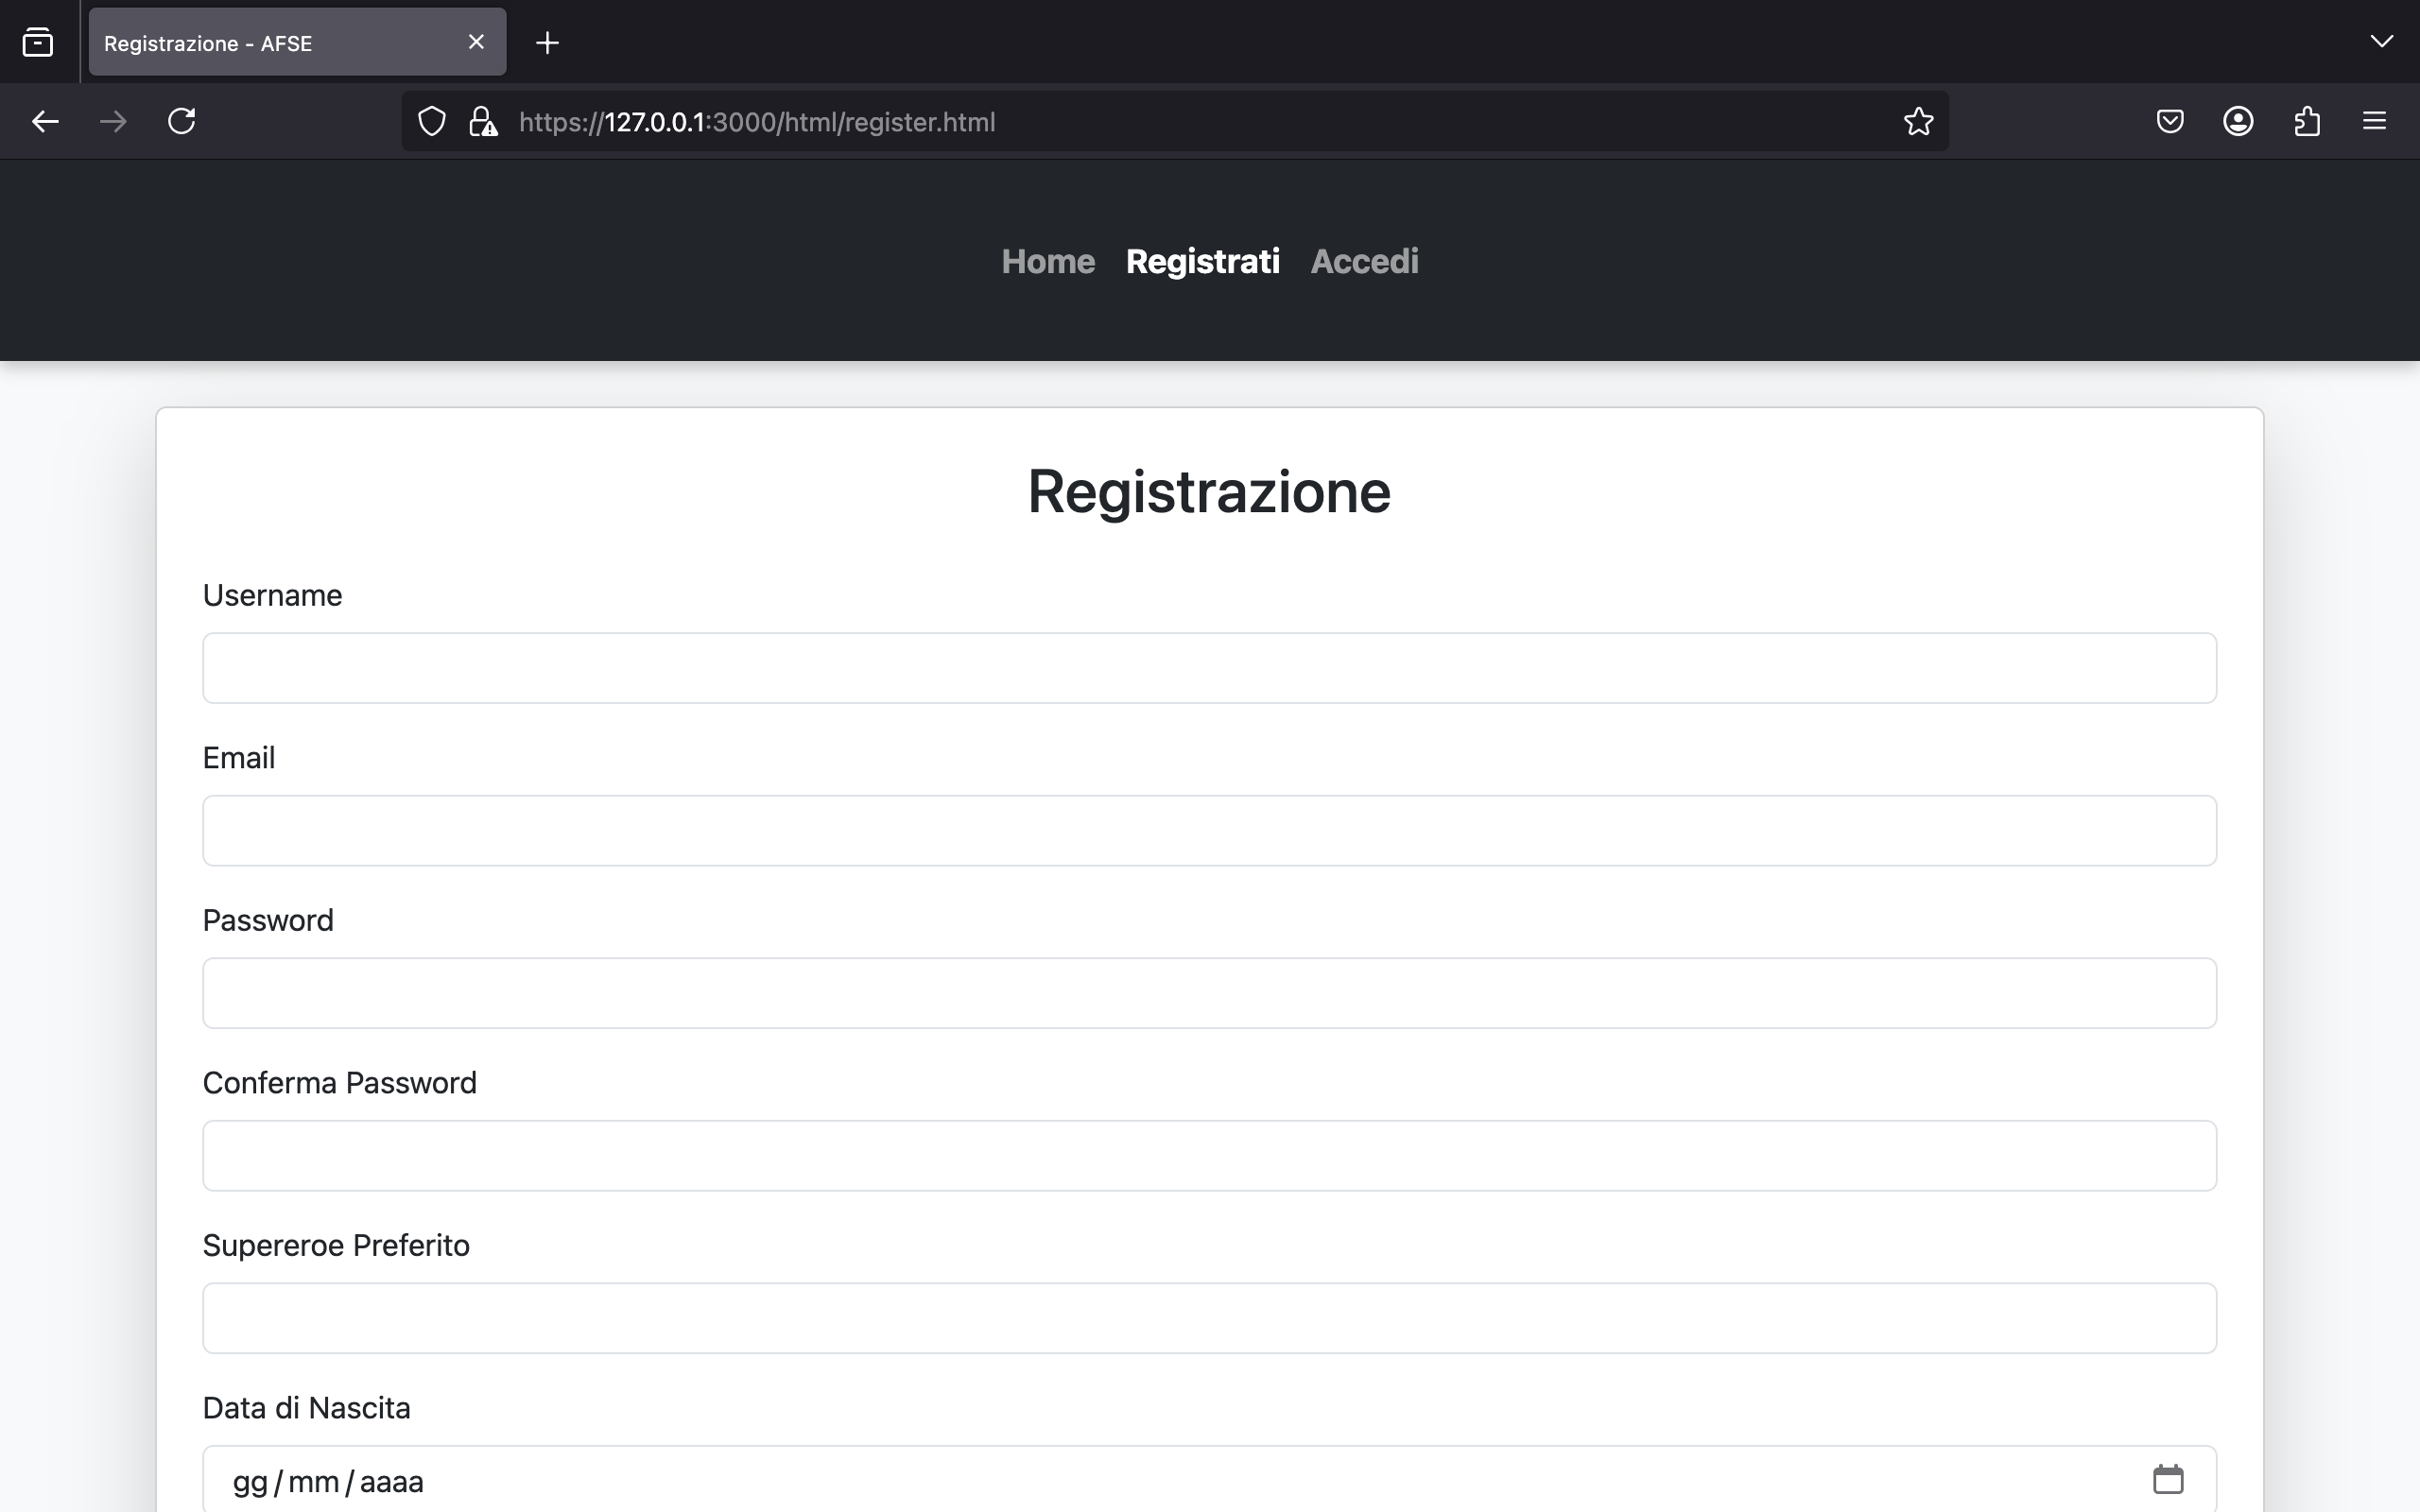
\includegraphics[width=\linewidth]{./content/registrazione.png}
        \end{minipage}

        \vspace{0.3cm} % Spazio tra le righe

        \begin{minipage}{0.3\linewidth}
            \centering
            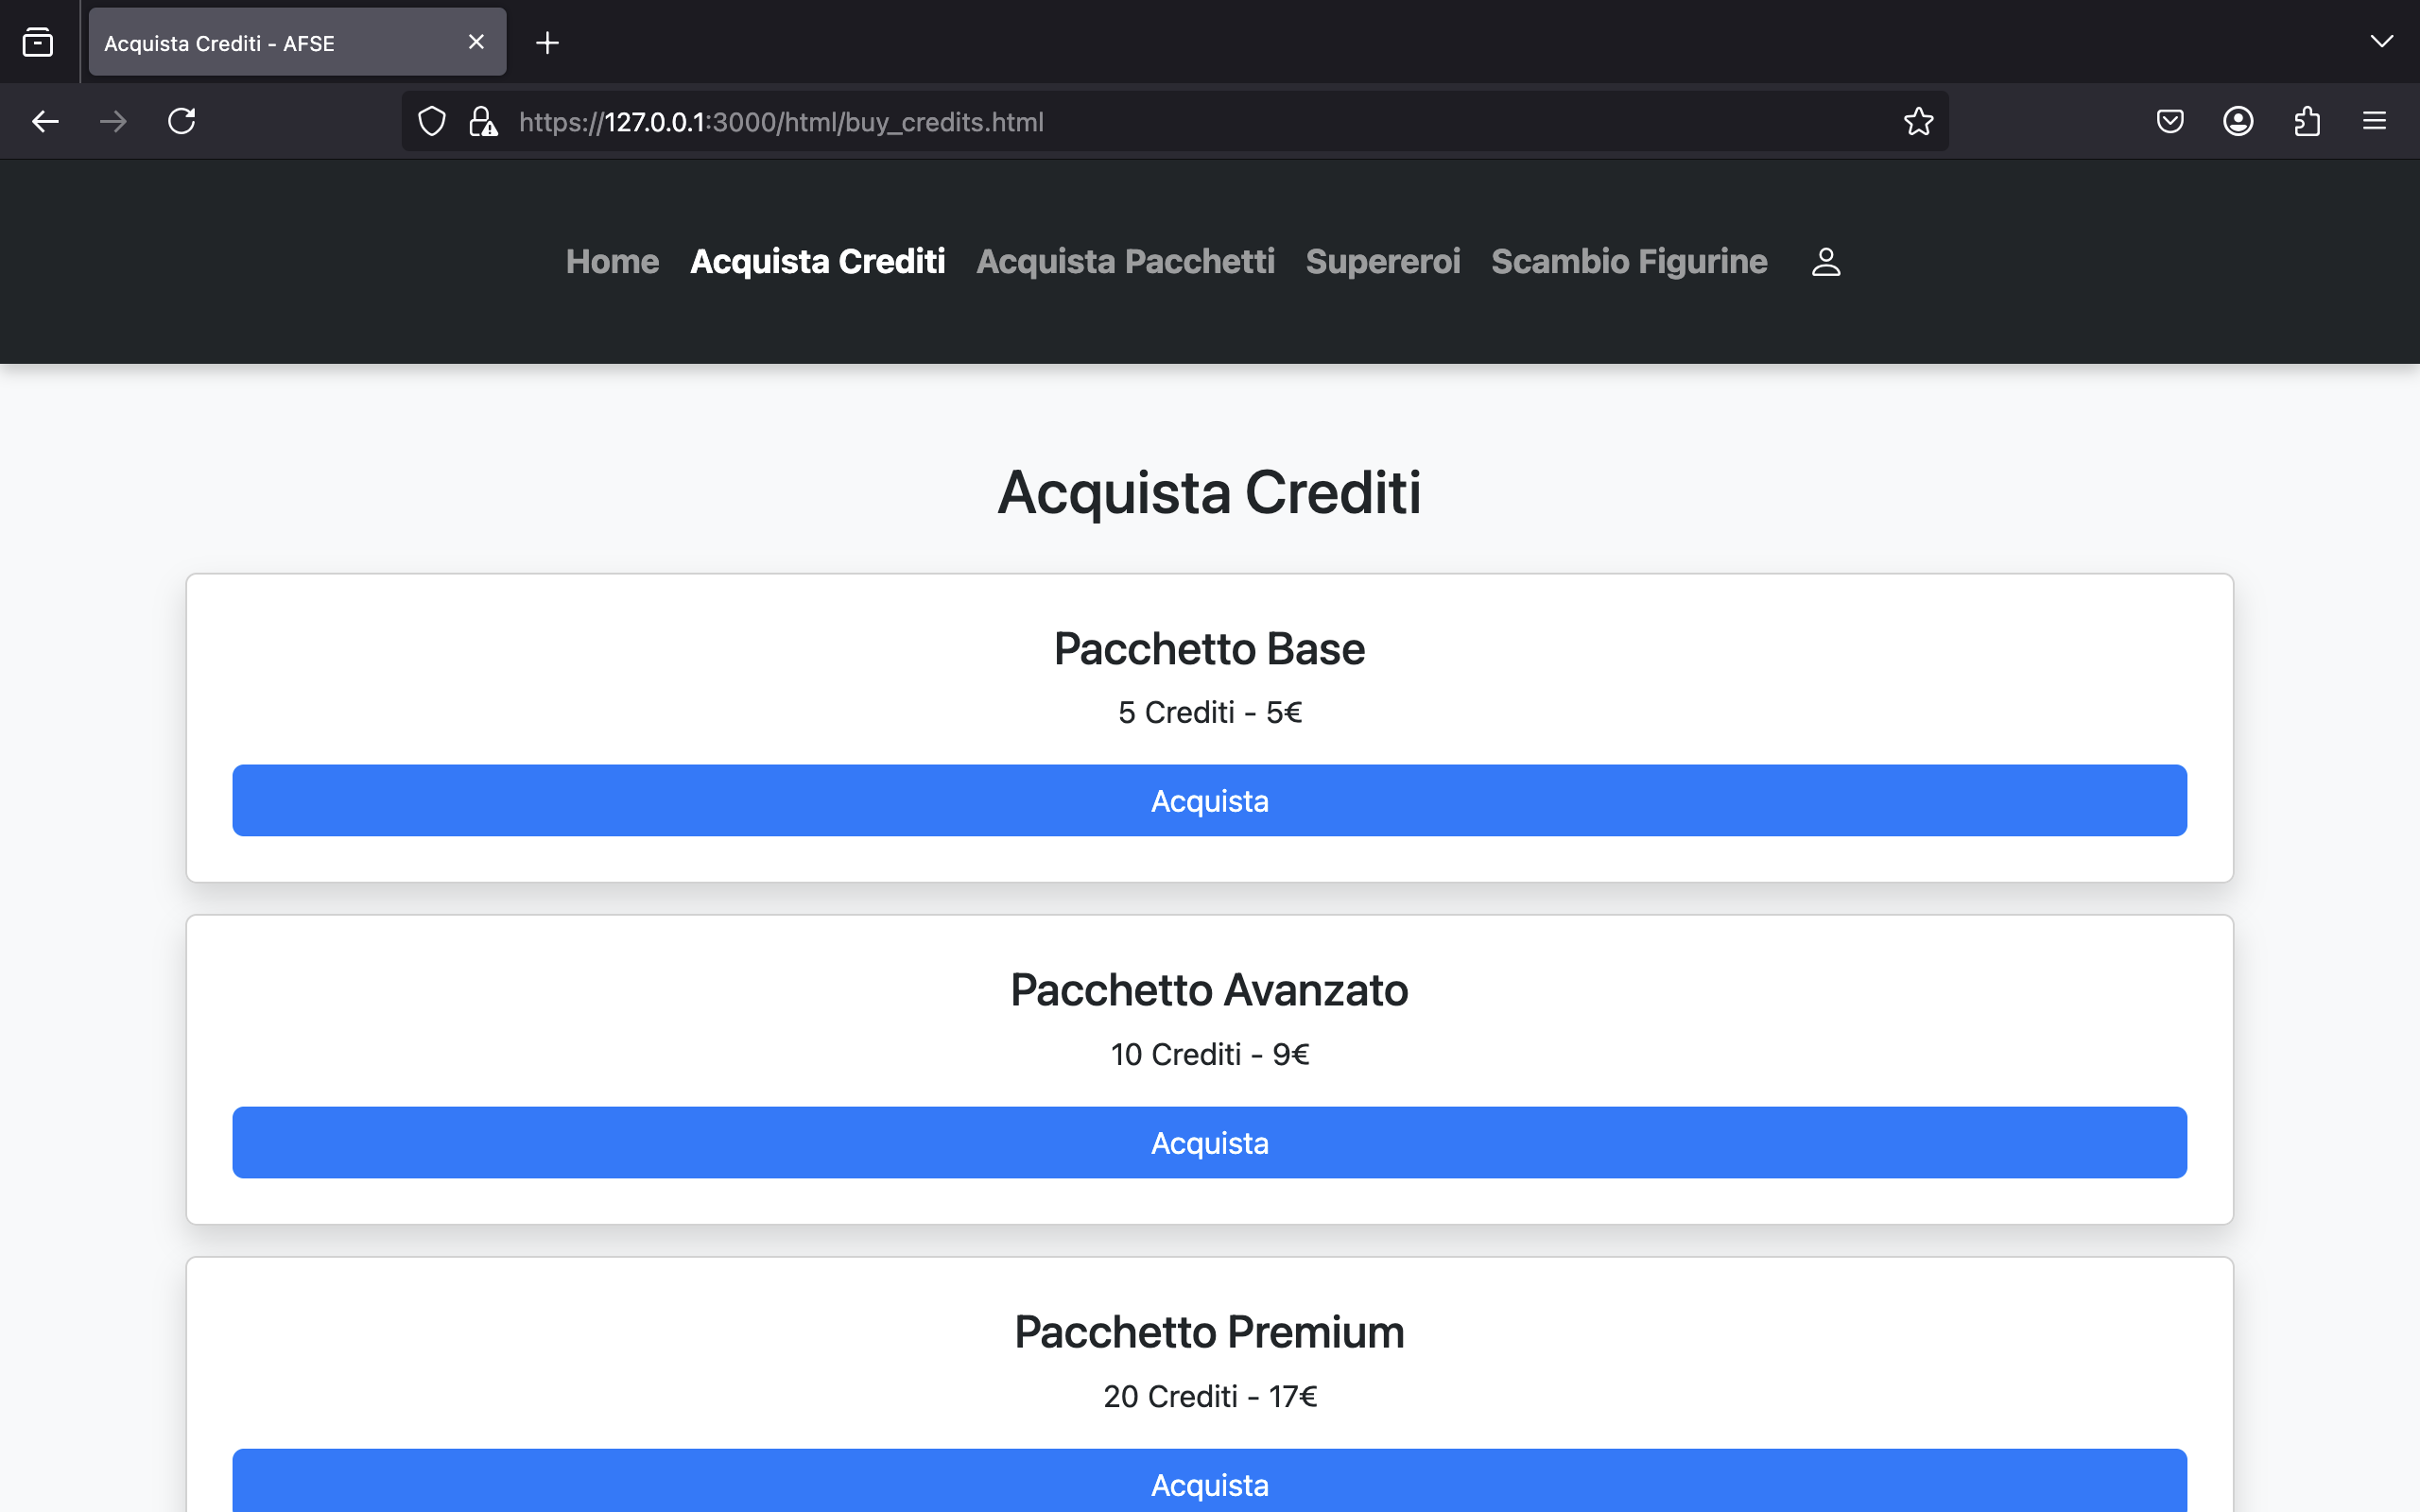
\includegraphics[width=\linewidth]{./content/crediti.png}
        \end{minipage}
        \hfill
        \begin{minipage}{0.3\linewidth}
            \centering
            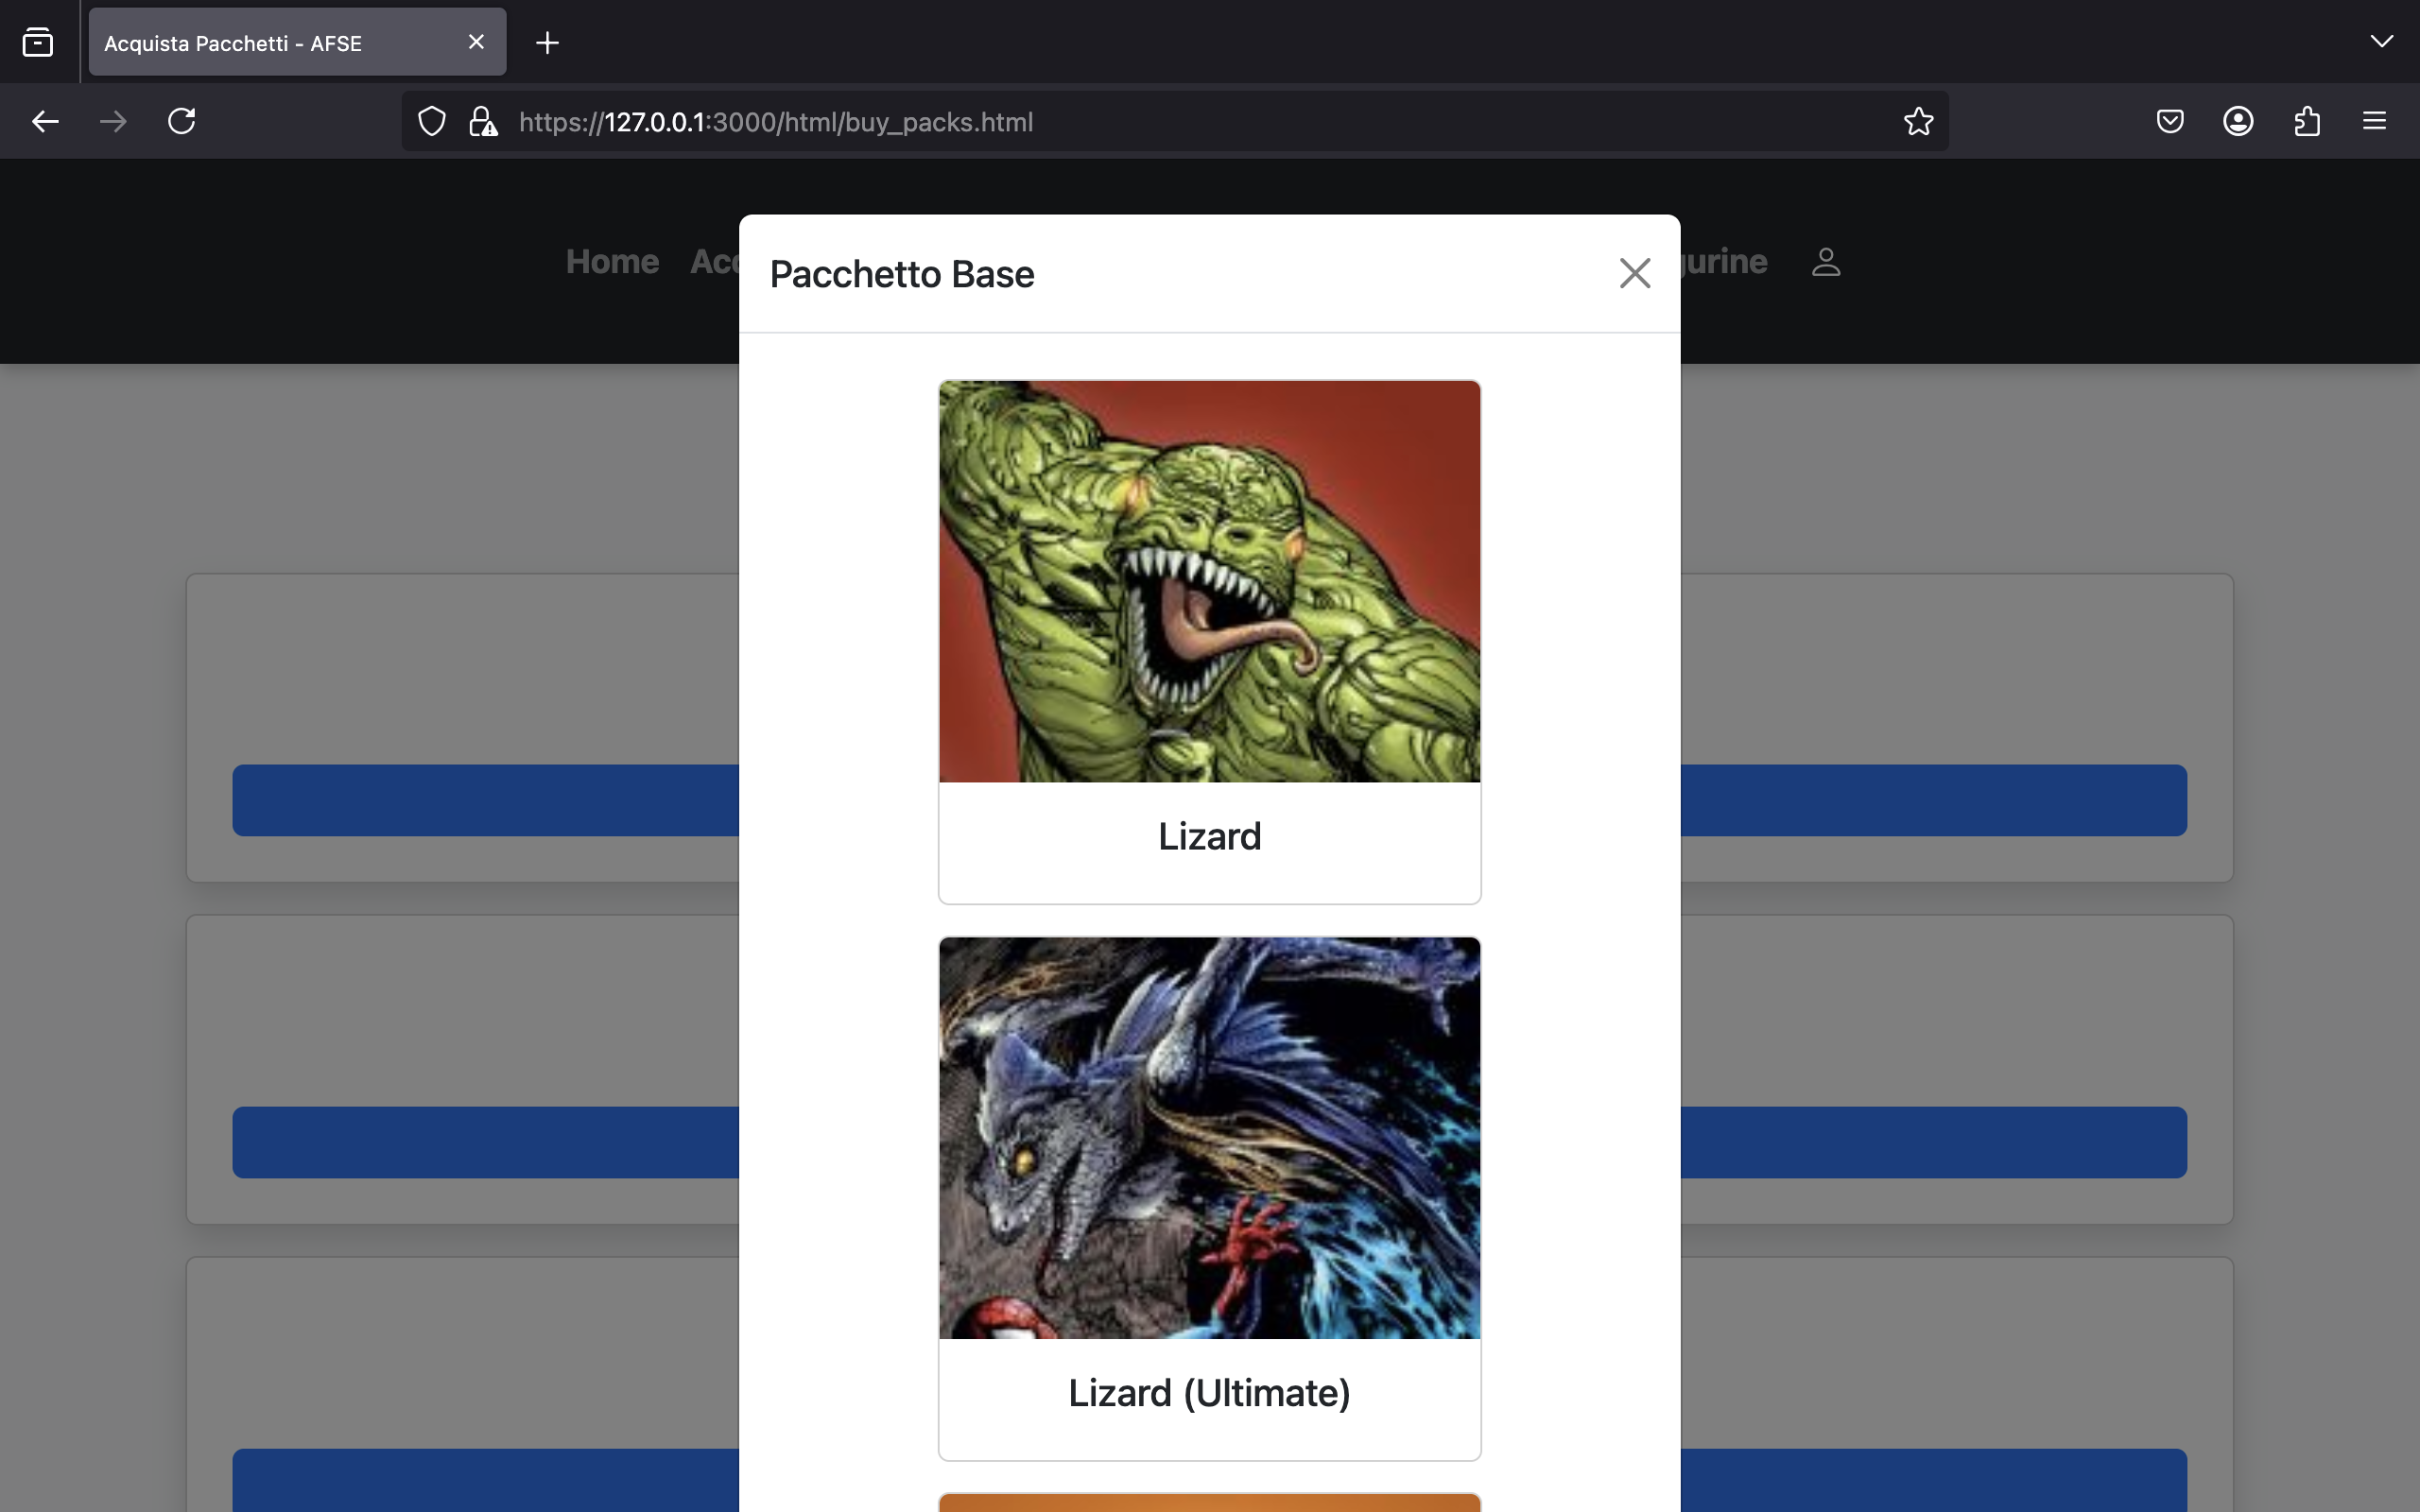
\includegraphics[width=\linewidth]{./content/pacchetto.png}
        \end{minipage}
        \hfill
        \begin{minipage}{0.3\linewidth}
            \centering
            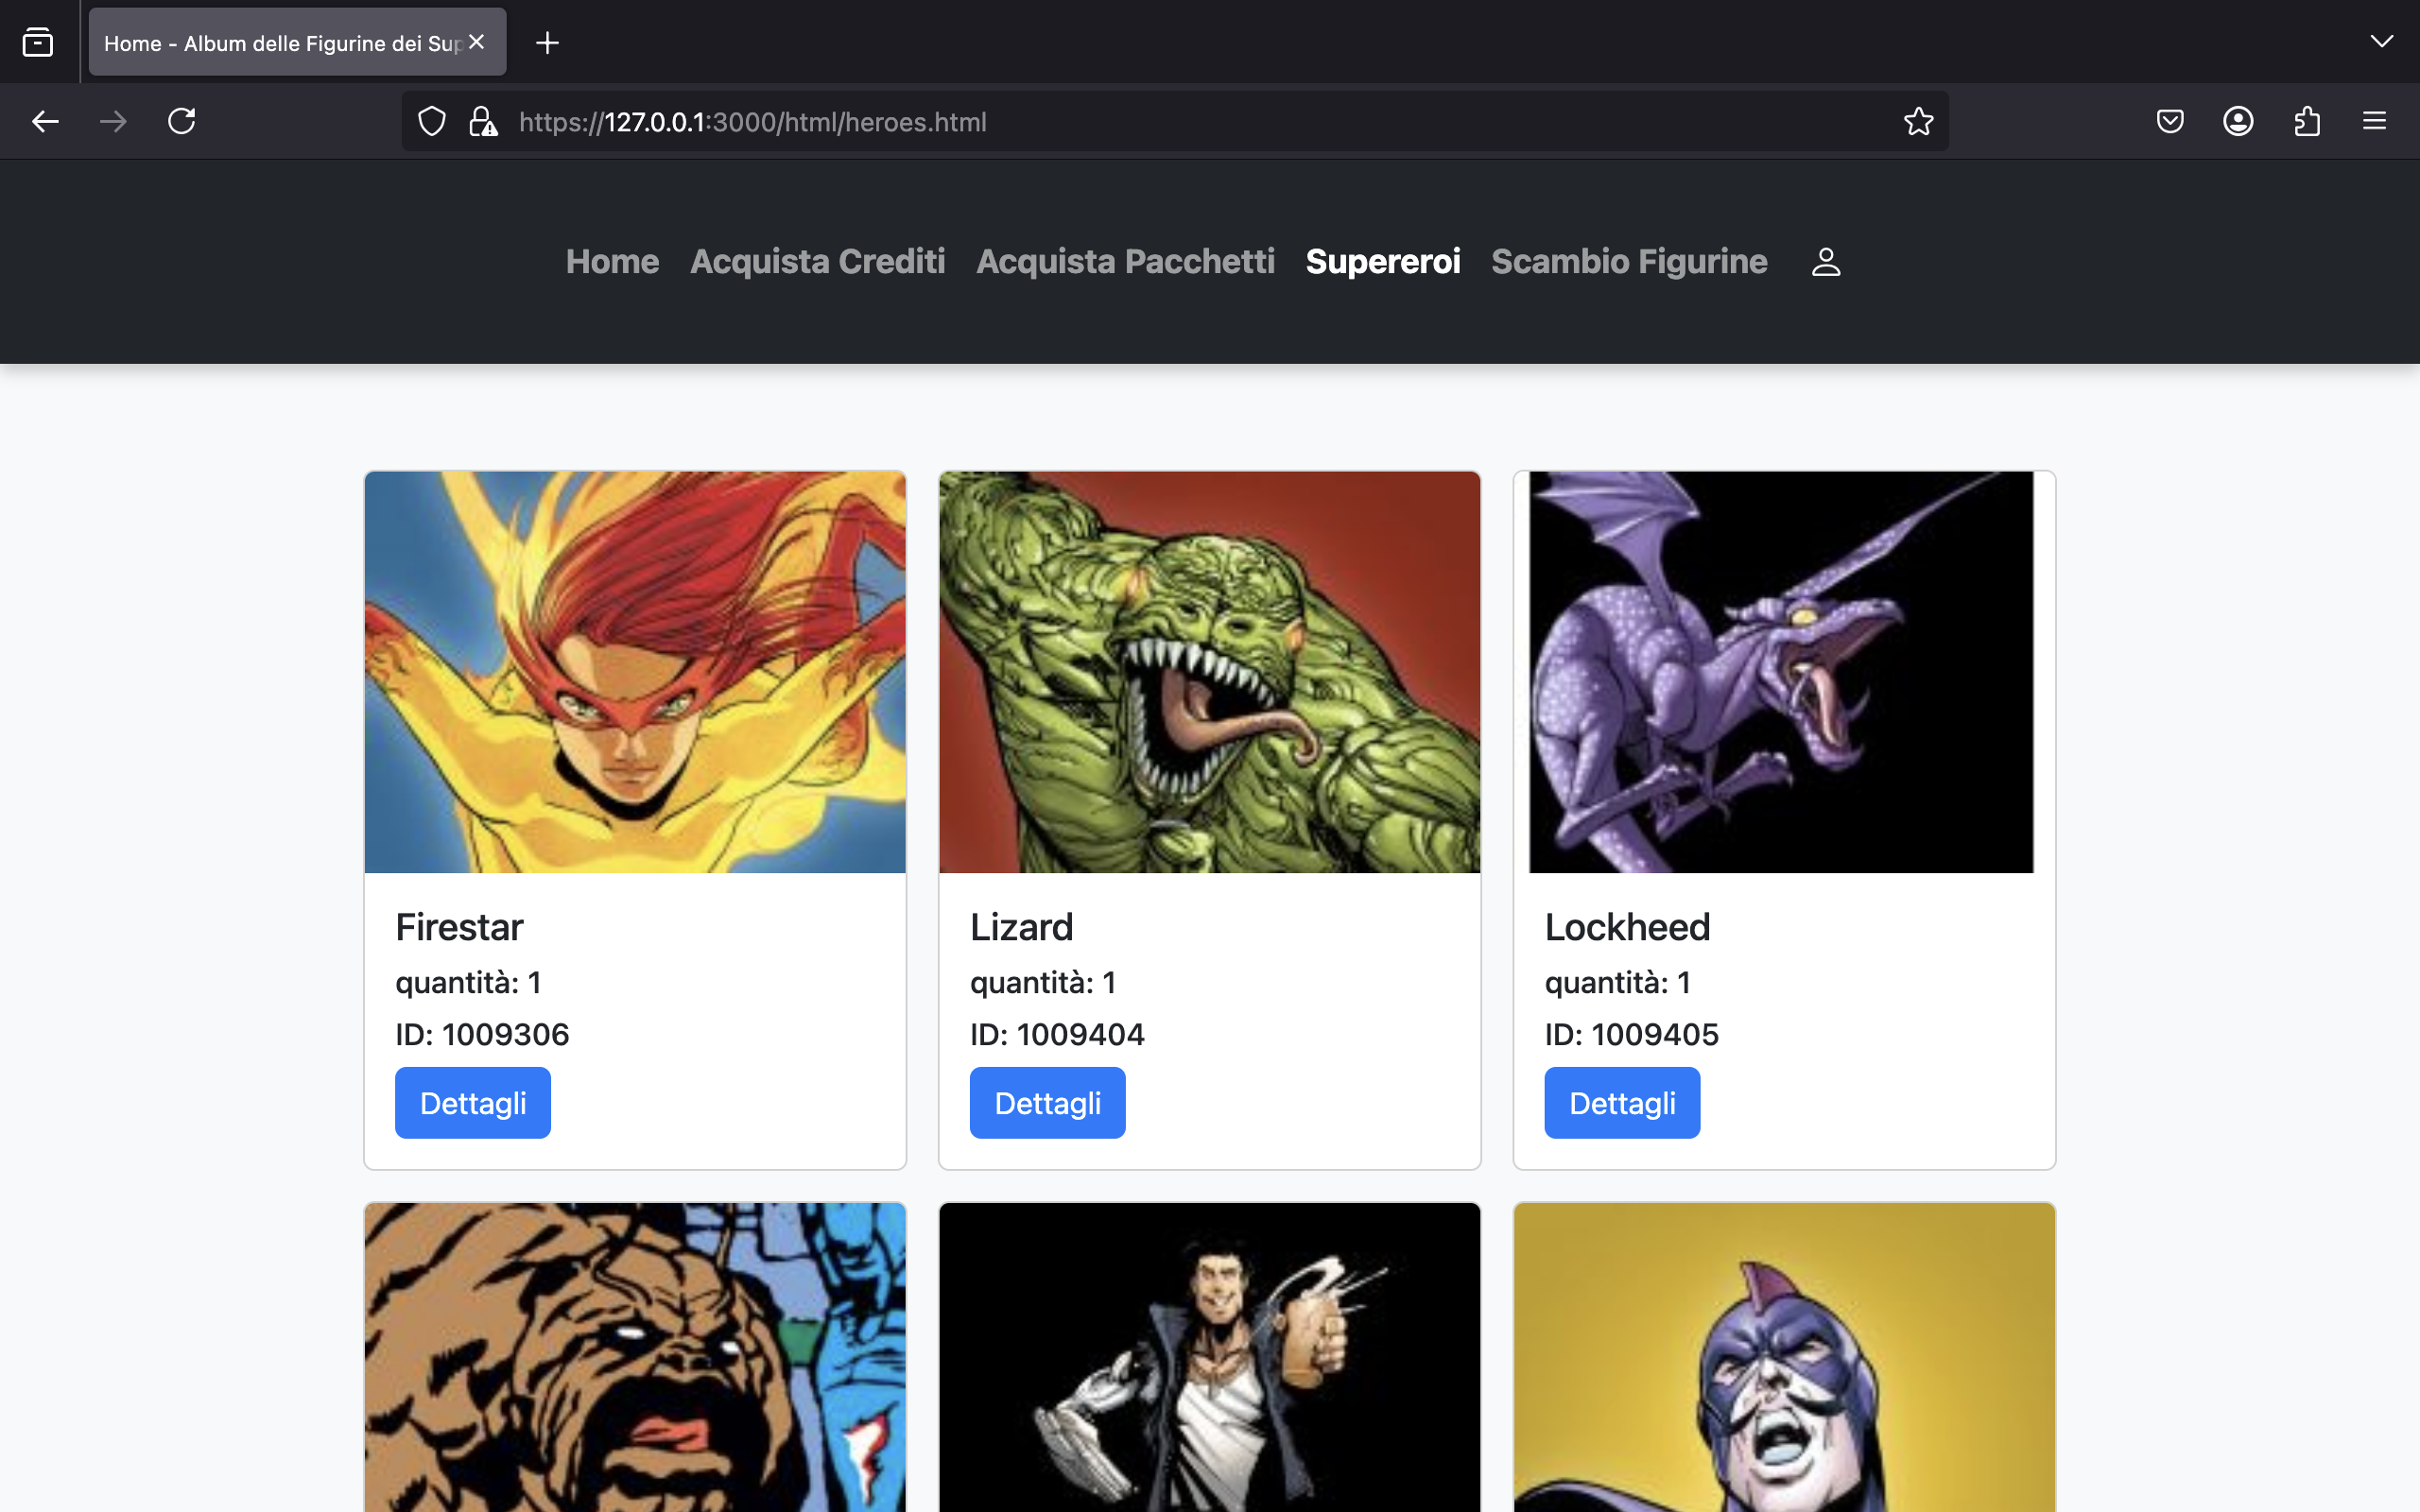
\includegraphics[width=\linewidth]{./content/album.png}
        \end{minipage}

        \vspace{0.3cm} % Spazio tra le righe

        \begin{minipage}{0.3\linewidth}
            \centering
            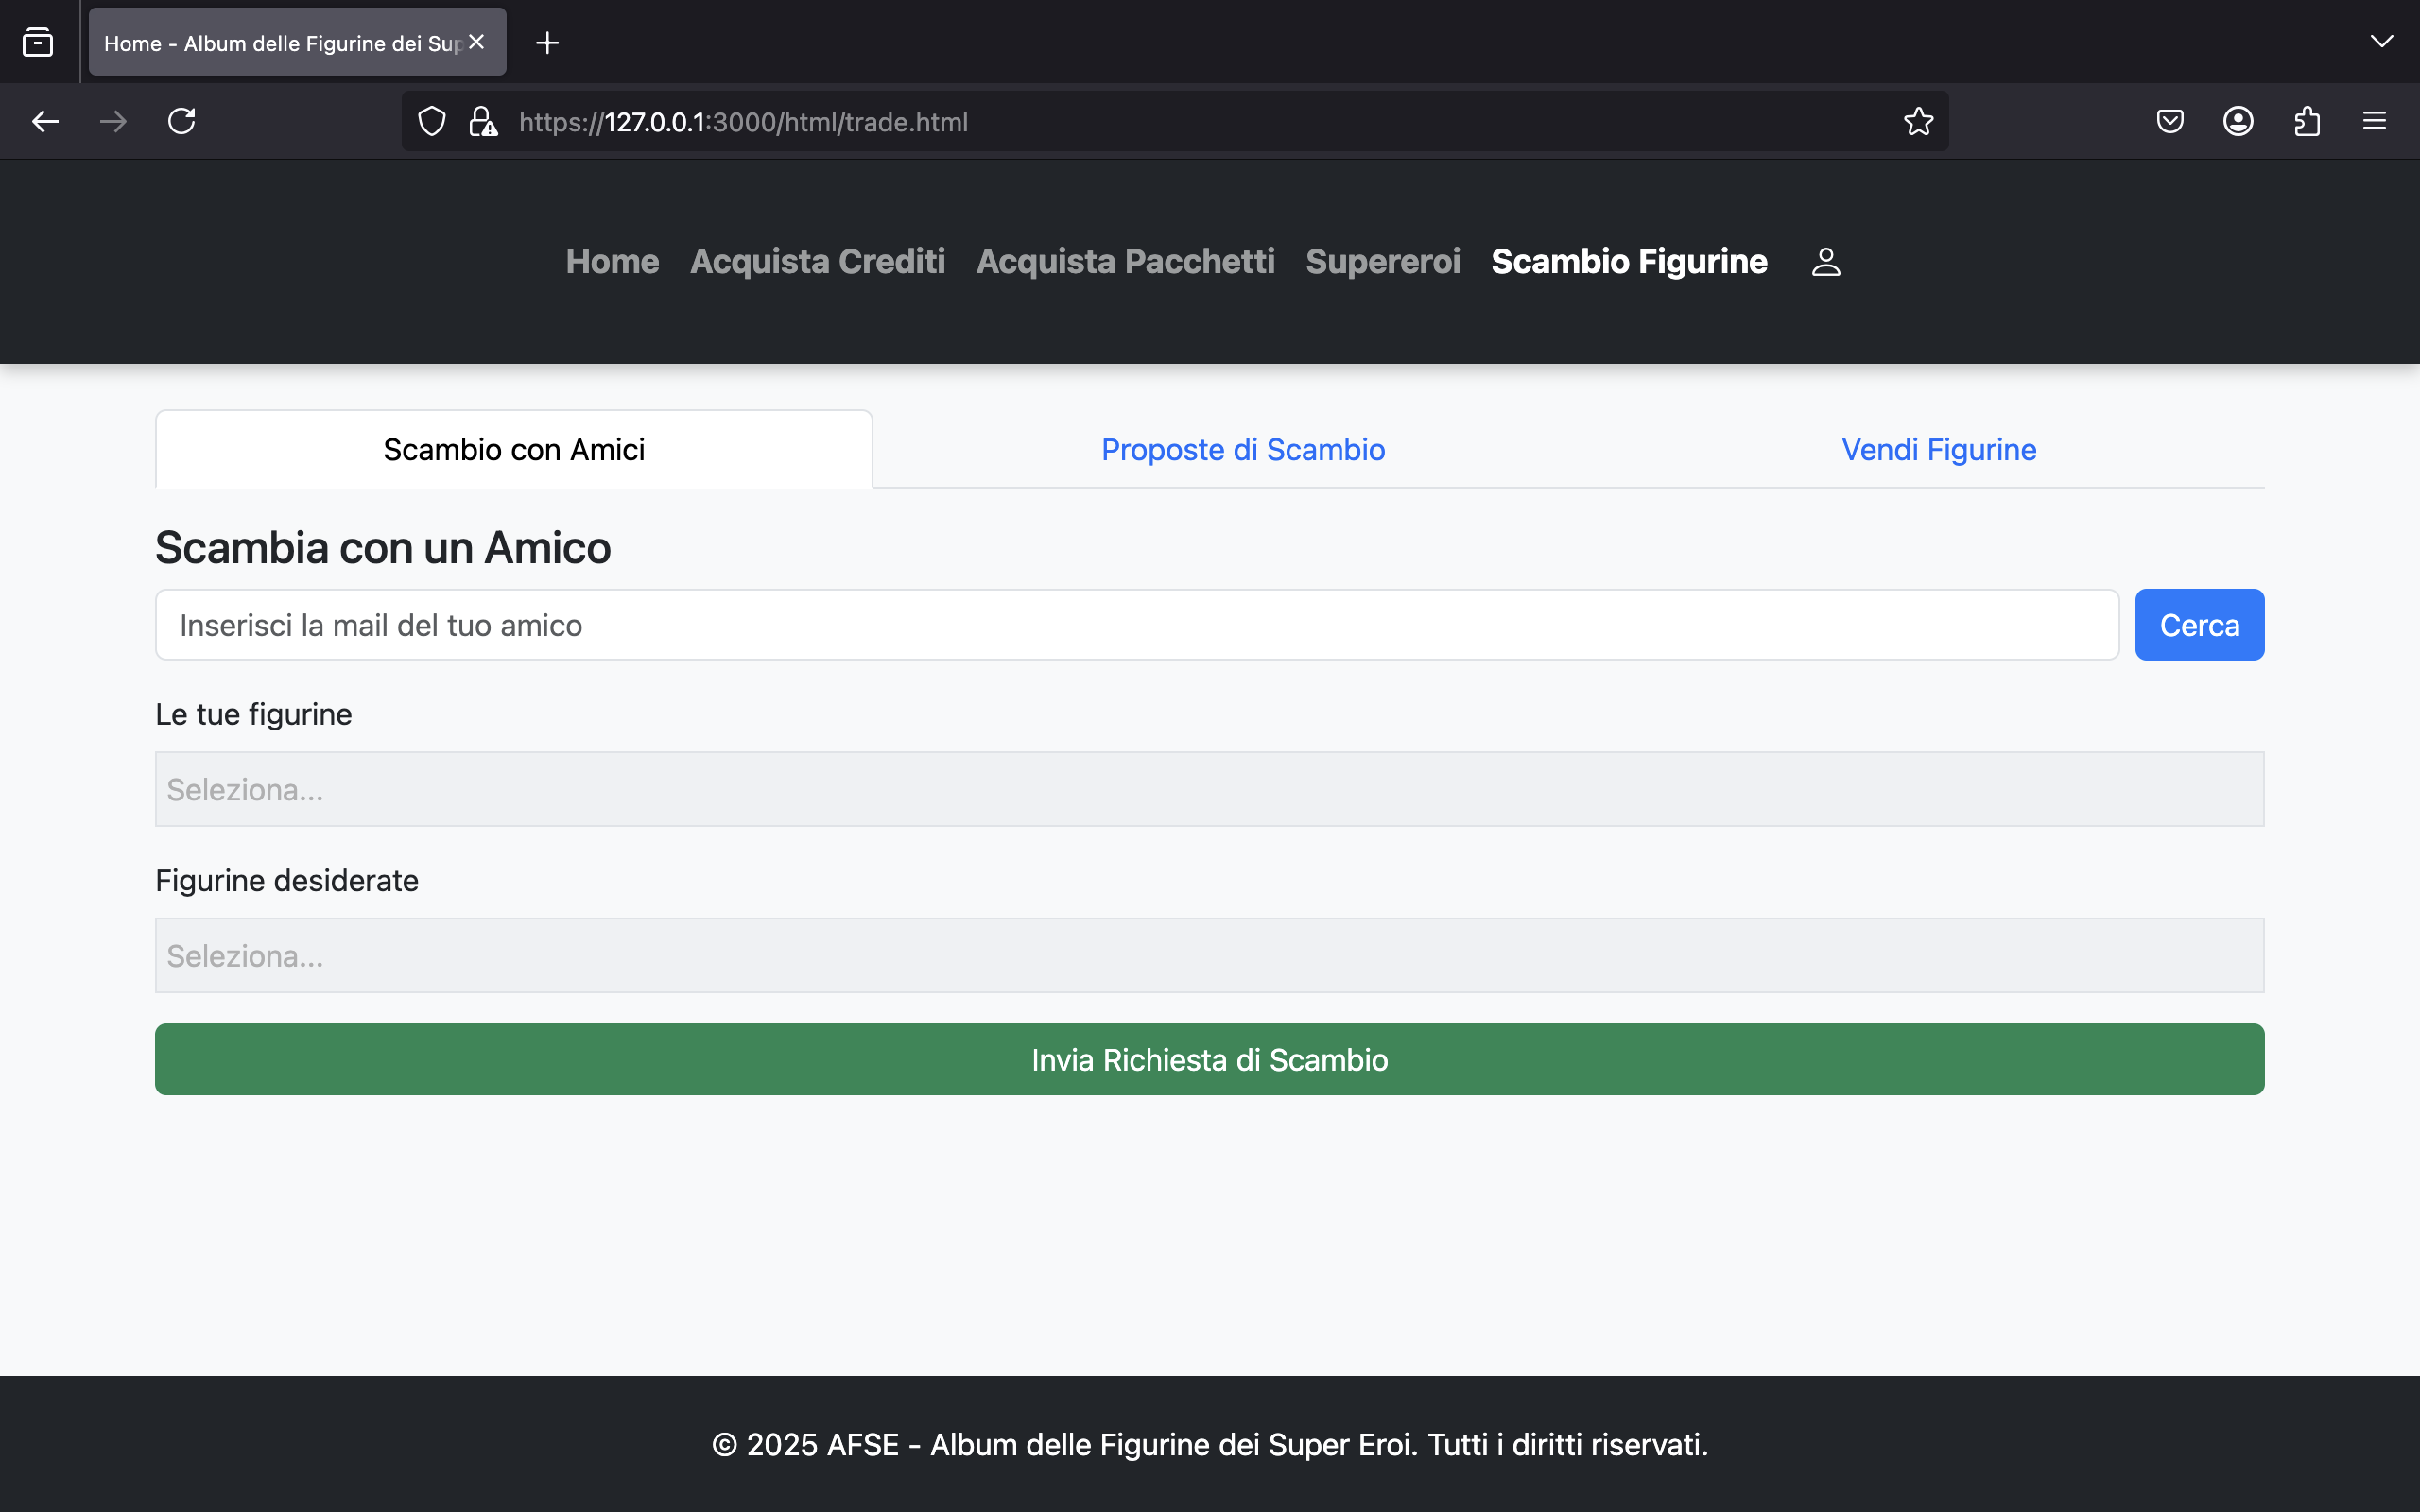
\includegraphics[width=\linewidth]{./content/scambio.png}
        \end{minipage}
        \hfill
        \begin{minipage}{0.3\linewidth}
            \centering
            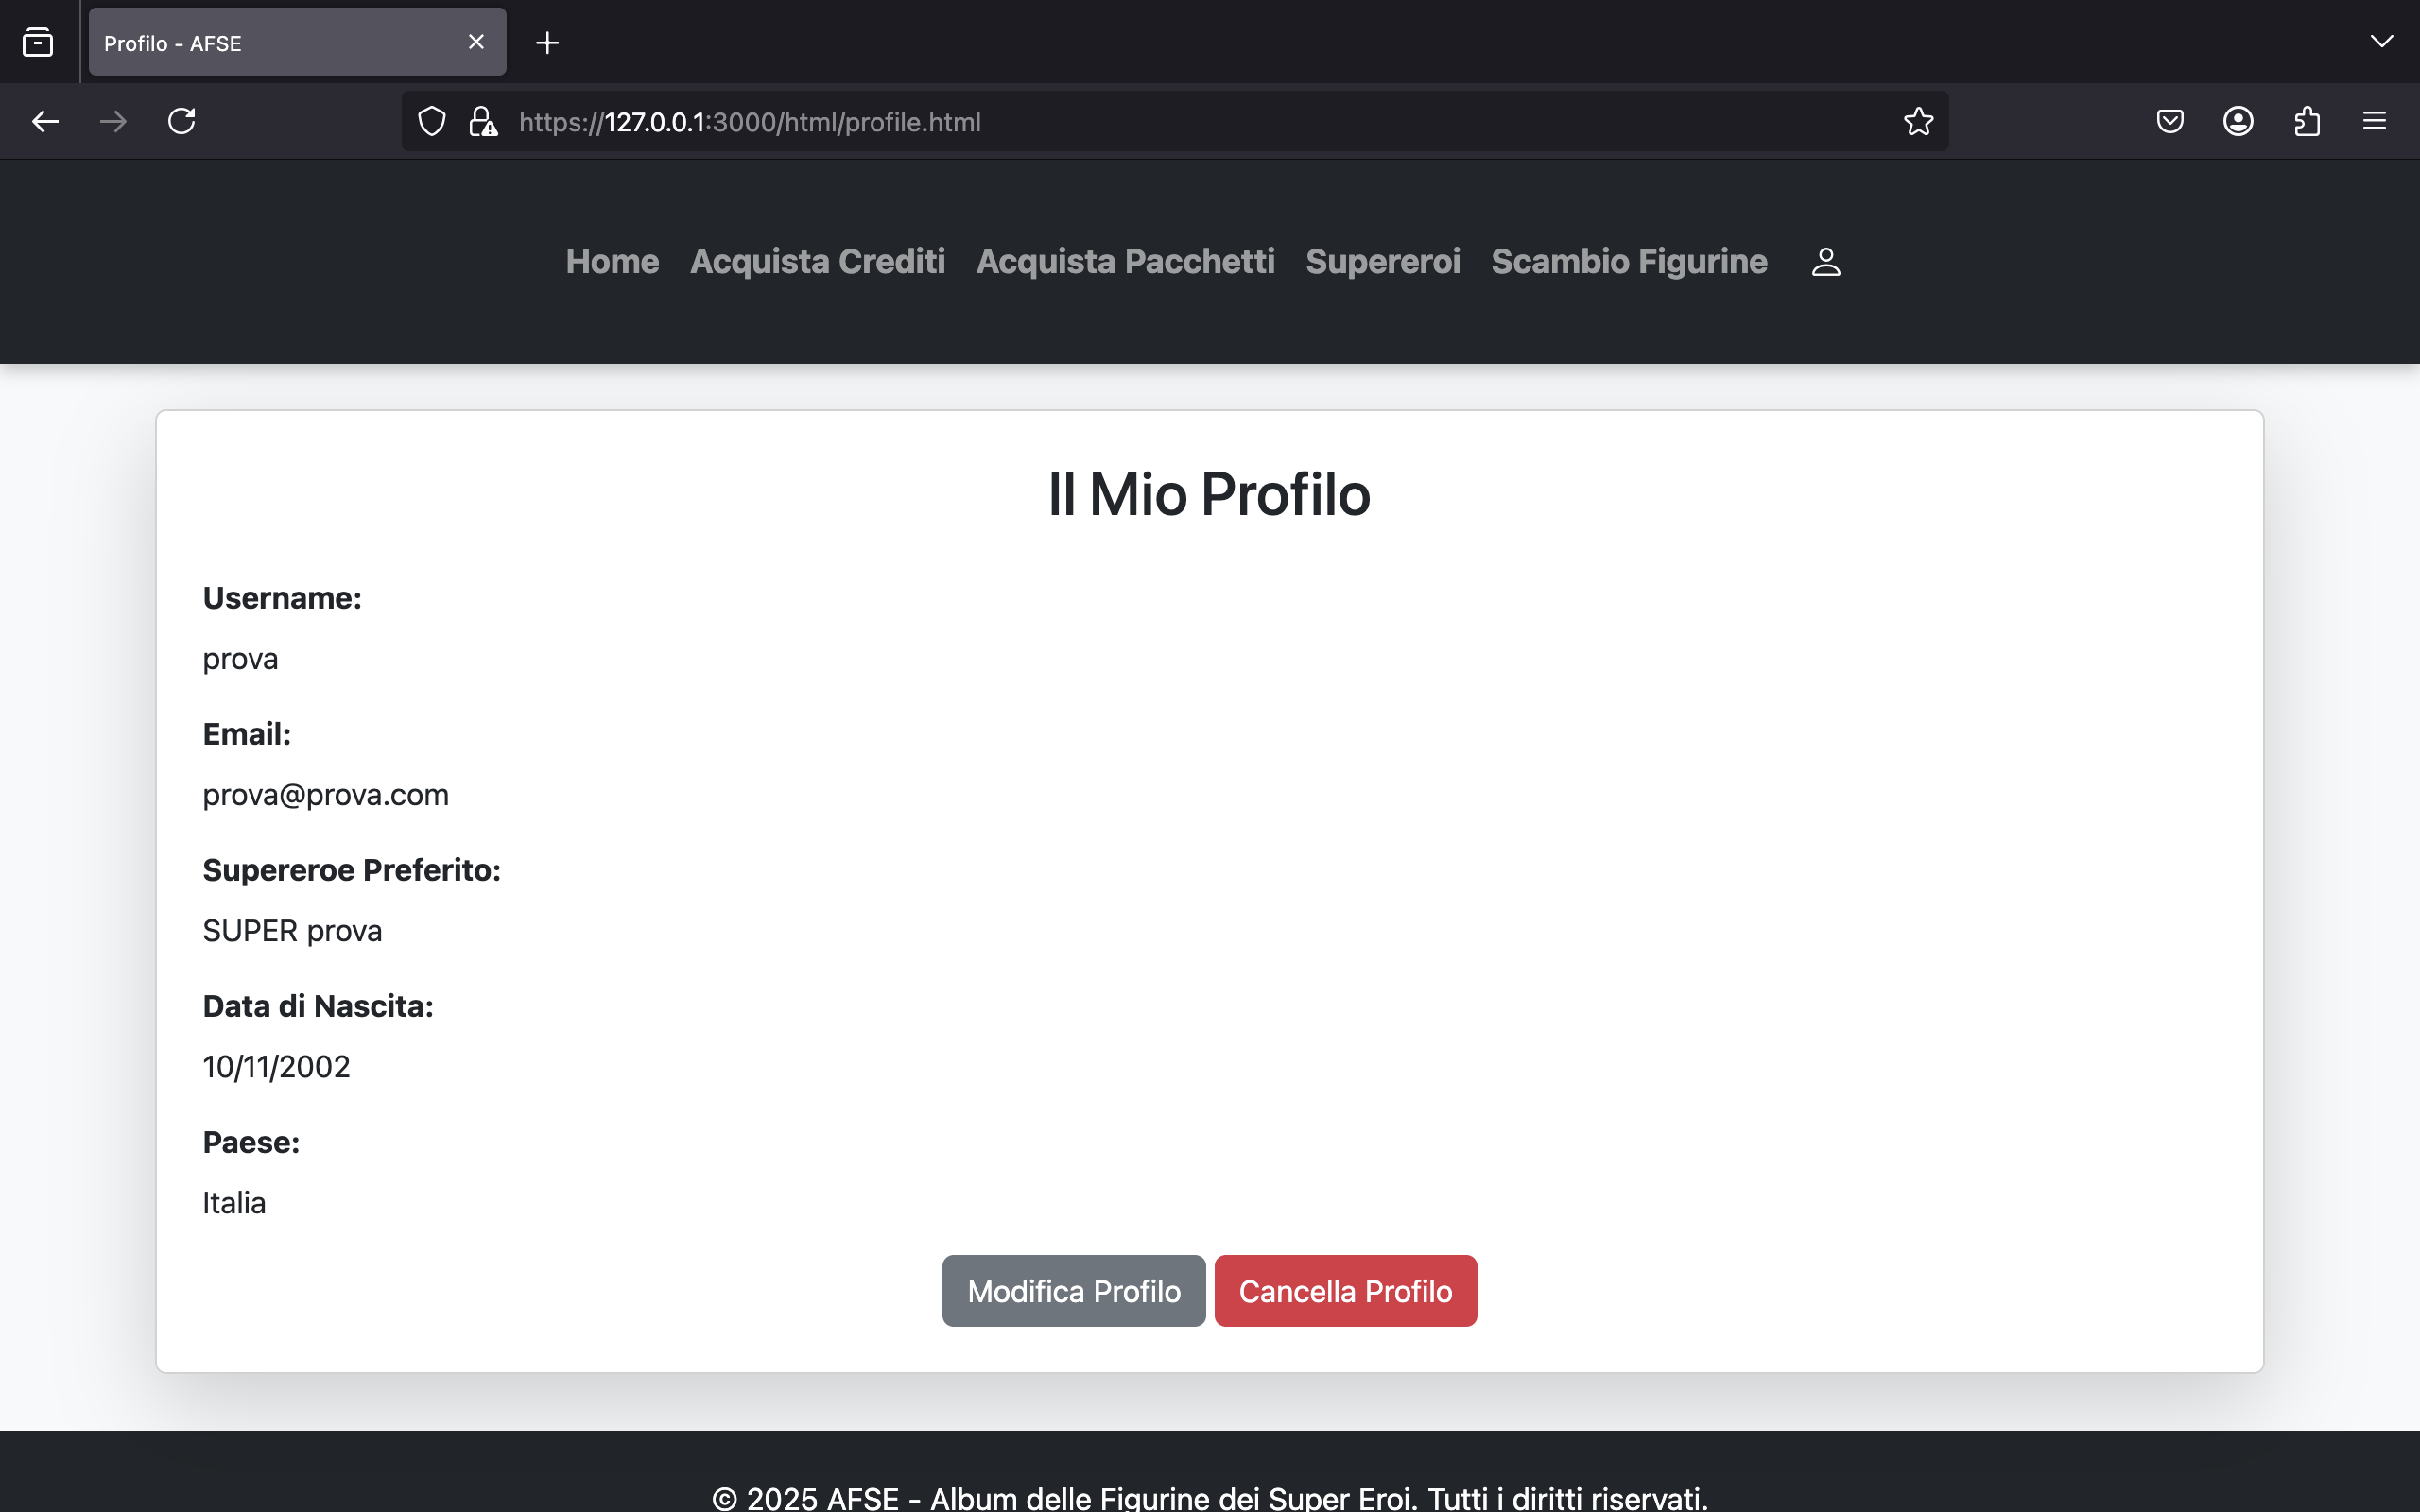
\includegraphics[width=\linewidth]{./content/profilo.png}
        \end{minipage}

    \end{figure}
\end{document}